In this chapter we will explore the technical requirements for integrating RTCWEB with a typical enterprise communications system architecture and give the suggested solution about the requirements. Then analyse some of the problems raised by the integration.

% Translation of bothe singaling and media is necessary.

\subsection{Integration}
Simple way:
Using SIP-over-WebSocket signaling and use an end-to-end media path enabled by \gls{wrtc}. This could work if the legacy enterprise system supported all the required protocols defined in \gls{wrtc}, otherwise the architecture would have to be upgraded to support all the new features. This is not trivial, since it would require to redo all of the existing architecture just to support \gls{wrtc}. It is better to create a bridge in the form of a gateway between \gls{wrtc} and the legacy architecture.

The gateway:

First showing a simple web application P2P WebRTC structure. Here signaling goes through a signaling server and media travels directly between the two peers(browsers).

\begin{figure}[here]
\centerline{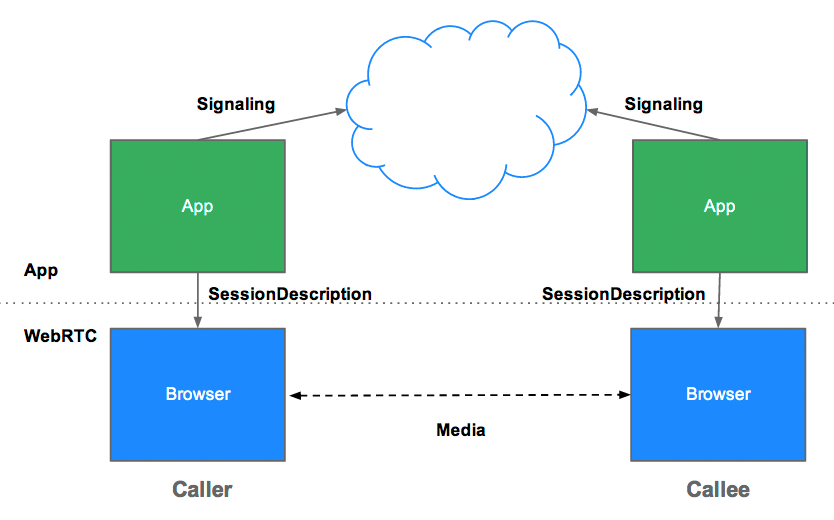
\includegraphics[scale=0.3]{jsep.png}}
\caption{WebRTC P2P architecture}
\label{fig:jsep}
\end{figure}

Secondly showing a typical enterprise architecture with signaling server, media server, and a server for routing the streams to peers.

\begin{figure}[here]
\centerline{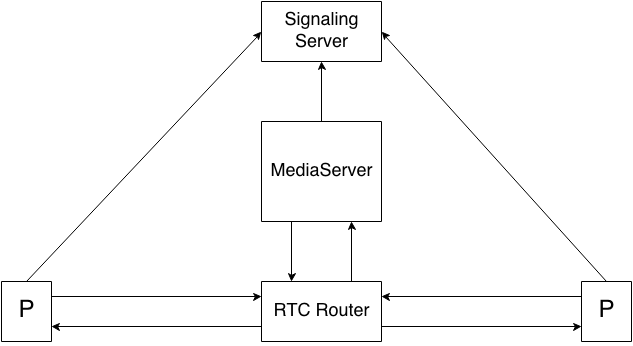
\includegraphics[scale=0.3]{VirtualArena.png}}
\caption{Enterprise communication platform architecture}
\label{fig:VirtualArenaArchitecture}
\end{figure}

Let's see how RTCWeb can be used to connect to existing enterprise communication networks.

In the solution figure we add an interworking gateway component. This component includes three subcomponents(signaling gateway, media relay gateway, and address server(address translation)). These provide all the necessary functionality.

%figure


\subsection{Summary}
The first iteration of RTCWeb is still under development, and not all protocols and codecs have been decided yet. It is theoretically possible to create a gateway and it has been done before under closed doors. Some of the biggest issues are how to handle the signaling, translating the media, and crossing the enterprise firewall.


% \subsection{Related Work}
% There is a great interest in interworking webRTC with existing telco services. An example is the integration with IMS. This work closely resembles the work that is done in this thesis. Currently there are gateway implemenations between webrtc and ims created by ericsson and mavenir. the 3gpp is doing work on drafting a standardized gateway implementation between webrtc and ims. Both ericsson and mavenir systems are closed to th epublic, but the 3gpp papers are open for reviewing.